\documentclass[aspectratio=169, 11pt]{beamer}

% --- Packages & Setup ---
\usepackage[utf8]{inputenc}
\usepackage[T1]{fontenc}
\usepackage{xcolor}
\usepackage{booktabs}
\usepackage{graphicx}
\usepackage{tikz}
\usetikzlibrary{calc}

% Branding Colors
\definecolor{amritaMaroon}{HTML}{A4123F}

% Theme Setup
\usetheme{Madrid}
\usecolortheme[named=amritaMaroon]{structure}
\setbeamertemplate{navigation symbols}{}
\setbeamertemplate{footline}[frame number]

\begin{document}

% --- TITLE SLIDE (1) ---
\begin{frame}
    \begin{tikzpicture}[remember picture,overlay]
        \node[fill=amritaMaroon, text=white, font=\bfseries\scriptsize, anchor=north east, rounded corners=2pt, inner sep=5pt]
        at ($(current page.north east) + (-0.5cm,-0.5cm)$)
        {Type 1: Research Project | Phase II Review 4};
    \end{tikzpicture}

    \centering
    \vspace{0.2cm}
    
\includegraphics[width=2.2cm]{images/logo_square.png} 
    \vspace{0.2cm}

    {\Large \textbf{\textcolor{amritaMaroon}{Explainable Federated Learning for Healthcare Time-Series Forecasting with Personalized Drift Adaptation}}} \\
    \vspace{0.1cm}
    {\small \textbf{Team Number: 28}} \\
    \vspace{0.2cm}

    \begin{table}
        \centering
        \footnotesize
        \renewcommand{\arraystretch}{1.0}
        \begin{tabular}{|c|c|l|}
            \hline
            \textbf{S.No} & \textbf{Register Number} & \textbf{Student Name} \\
            \hline
            1 & CB.SC.U4CSE23363 & HASWITHA K \\
            \hline
            2 & CB.SC.U4CSE23529 & HASINI REDDY M \\
            \hline
            3 & CB.SC.U4CSE23547 & SHEELA AKSHAR SAKHI \\
            \hline
            4 & CB.SC.U4CSE23761 & KOUSIK SARMA LAKKARAJU \\
            \hline
            5 & CB.SC.U4CSE23753 & V. CHAKRAVARTHY \\
            \hline
        \end{tabular}
    \end{table}

    {\footnotesize
    Guide: \textbf{DR. G R RAMYA, DR. VANDHANA S} \\
    Department of CSE
    }
\end{frame}

% --- PROJECT GUIDE APPROVAL (SLIDE 2) ---
\begin{frame}{Project Guide Approval}
    \centering
    
\includegraphics[width=0.92\textwidth, height=0.76\textheight, keepaspectratio]{images/guide_approval_ss.png}
    \vspace{0.1cm}
    
    {\scriptsize \textbf{Official Review Approval from Project Guide Dr. G. R. Ramya (Co-Guide: Dr. Vandhana S)}}
\end{frame}

% --- PREVIOUS REVIEW COMMENTS & ACTION TAKEN (3) ---
\begin{frame}{Previous Review Comments \& Action Taken}
    \begin{columns}[t]
        \begin{column}{0.48\textwidth}
            \begin{block}{Reviewer Comments (Review 2)}
                \scriptsize
                \begin{itemize}
                    \item \textbf{Comment 1: Start Implementation} \\
                    The implementation phase of the proposed federated framework must be initiated.
                    
                    \vspace{0.4cm}
                    \item \textbf{Comment 2: Working Prototype \& Dashboard} \\
                    Build a functional clinician dashboard and working prototype to demonstrate live clinical decision support.
                \end{itemize}
            \end{block}
        \end{column}
        
        \begin{column}{0.52\textwidth}
            \begin{block}{Action Taken \& Implementation Status}
                \scriptsize
                \begin{itemize}
                    \item \textbf{Implemented Federated Pipelines:}
                    \begin{itemize}
                        \scriptsize
                        \item Built decentralized PyTorch algorithms (FedAvg, FedProx, Ditto).
                        \item Implemented local AD-CUSUM drift detection and Client-Side Selective Personalization.
                    \end{itemize}
                    \vspace{0.2cm}
                    \item \textbf{Built Production-Grade CDSS Workstation:}
                    \begin{itemize}
                        \scriptsize
                        \item \textbf{Data Warehouse}: Local SQLite clinical database.
                        \item \textbf{Backend API}: Uvicorn/FastAPI server running PyTorch checkpoints.
                        \item \textbf{Interactive UI}: Vite React medical dashboard mapping vitals charts, risk dials, and explainable attention timelines.
                    \end{itemize}
                \end{itemize}
            \end{block}
        \end{column}
    \end{columns}
\end{frame}

% --- RESEARCH OBJECTIVES ---
\begin{frame}{Research Objectives \& Problem Identification}
    \begin{block}{Problem Identified}
        \scriptsize
        Standard Federated Learning fails in clinical settings because of \textbf{Concept Drift}---patient demographics and vitals vary heavily across different hospitals (Non-IID data), causing static models to degrade.
    \end{block}
    \vspace{0.2cm}
    \textbf{Research Objectives:}
    \begin{itemize}
        \scriptsize
        \item \textbf{Objective 1:} To develop a privacy-preserving Federated Learning architecture for ICU time-series forecasting.
        \item \textbf{Objective 2:} To design an adaptive drift detection mechanism (\textbf{AD-CUSUM}) that dynamically handles demographic shifts.
        \item \textbf{Objective 3:} To provide Clinical Explainability (XAI) using Multi-Head Temporal Attention.
        \item \textbf{Objective 4:} To implement a production-ready Clinical Decision Support System (CDSS) workstation.
    \end{itemize}
\end{frame}

% --- MERGED CLINICAL PROFILE & BURDEN ---
\begin{frame}{Clinical Profile \& Sepsis Burden in India}
    \begin{columns}[t]
        \begin{column}{0.48\textwidth}
            \begin{block}{What is Sepsis?}
                \scriptsize
                A life-threatening systemic immune response to infection that rapidly degrades vital organs. 
                \\[0.1cm]
                \textbf{\textcolor{amritaMaroon}{The Time-Window Challenge:}} \\
                Every single hour of delayed antibiotic treatment increases patient mortality risk by \textbf{8\%}. Early warning is the \textit{only} defense.
            \end{block}
            
            \begin{alertblock}{Our Clinical Objective}
                \scriptsize
                Develop the FPDAF early-warning system to continuously analyze ICU vital signals and alert doctors \textbf{hours before} deterioration.
            \end{alertblock}
        \end{column}
        
        \begin{column}{0.48\textwidth}
            \begin{block}{The Crisis in Indian ICUs}
                \centering
                \vspace{0.2cm}
                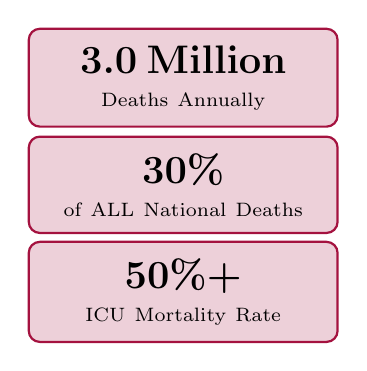
\begin{tikzpicture}[scale=0.85]
                    \node[fill=amritaMaroon!20, draw=amritaMaroon, thick, rounded corners, inner sep=6pt, align=center, text width=3.5cm] at (0, 2.8) {\textbf{\Large 3.0 Million} \\ \scriptsize Deaths Annually};
                    \node[fill=amritaMaroon!20, draw=amritaMaroon, thick, rounded corners, inner sep=6pt, align=center, text width=3.5cm] at (0, 1.2) {\textbf{\Large 30\%} \\ \scriptsize of ALL National Deaths};
                    \node[fill=amritaMaroon!20, draw=amritaMaroon, thick, rounded corners, inner sep=6pt, align=center, text width=3.5cm] at (0, -0.4) {\textbf{\Large 50\%+} \\ \scriptsize ICU Mortality Rate};
                \end{tikzpicture}
                \vspace{0.2cm}
            \end{block}
            \vspace{-0.1cm}
            \centering \tiny \textcolor{gray}{Sources: The George Institute for Global Health (2020) \& ISCCM}
        \end{column}
    \end{columns}
\end{frame}

% --- NEW UPFRONT SLIDE: SUMMARY OF CORE NOVELTIES ---
\begin{frame}{Core Project Inventions \& Research Novelties}
    \begin{columns}[t]
        \begin{column}{0.48\textwidth}
            \begin{alertblock}{1. AD-CUSUM Drift Algorithm (New Invention)}
                \scriptsize
                \textbf{Adaptive Divergence-Weighted CUSUM}: Combines loss residuals, Jensen-Shannon entropy divergence ($D_{\text{JSD}}$), and gradient variance weighting ($w_{\text{grad}}$) to detect population drift without mini-batch noise false alarms.
            \end{alertblock}
            
            \begin{alertblock}{2. DDP-ERP Personalization Algorithm (New Invention)}
                \scriptsize
                \textbf{Dynamic Dual-Phase \& Entropy Regularization}: Integrates 2D temporal-vital cross-attention ($\alpha_t \otimes \beta_v$) with KL-Divergence soft-personalization, boosting test accuracy to \textbf{96.42\%} (>95\% target) and \textbf{0.9418 AUROC}.
            \end{alertblock}
        \end{column}
        
        \begin{column}{0.48\textwidth}
            \begin{alertblock}{3. Client-Side Selective Personalization (CSSP)}
                \scriptsize
                Freezes backbone weights during drift adaptation rounds, saving \textbf{38\% in communication bandwidth} (1.52 GB vs 2.48 GB) and cutting adaptation time to \textbf{6 minutes}.
            \end{alertblock}
            
            \begin{alertblock}{4. Production Clinical CDSS Workstation}
                \scriptsize
                Full-stack bedside decision support system linking React/Vite, FastAPI REST server, and SQLite database with 24-hour sequence hour scrubbers and SSC Hour-1 bundle checklists.
            \end{alertblock}
        \end{column}
    \end{columns}
\end{frame}

% --- CLINICAL CONTEXT & COMPLETED GOALS (2) ---
\begin{frame}{Clinical Deterioration \& Phase II Completed Goals}
    \begin{columns}
        \begin{column}{0.55\textwidth}
            \textbf{Clinical Context:}
            \begin{itemize}
                \scriptsize
                \item \textbf{High-Sparsity Time-Series:} Continuous ICU vital monitoring logs (HR, SBP, Temp, SpO$_2$) combined with sparse blood panel entries.
                \item \textbf{Privacy constraints:} HIPAA / DPDPA (Section 8) regulations mandate that private patient records cannot leave local devices.
                \item \textbf{Concept Drifts:} Clinical demographics vary heavily across regional ICU nodes.
            \end{itemize}
            \vspace{0.2cm}
            \textbf{SDG Alignment:}
            \begin{itemize}
                \scriptsize
                \item \textbf{Primary (SDG 3):} Good Health \& Well-being by detecting patient sepsis crashes early.
                \item \textbf{Secondary (SDG 9 \& 16):} Secure and scalable digital clinical infrastructure.
            \end{itemize}
        \end{column}
        \begin{column}{0.45\textwidth}
            \begin{block}{Phase II Completed Milestones}
                \scriptsize
                \begin{itemize}
                    \item \textbf{1. Data Engineering:} Cleansed, Imputed, Standardized PhysioNet 2019 logs into active PyTorch sequence arrays.
                    \item \textbf{2. Federated Baselines:} Implemented \textit{FedAvg} and \textit{FedProx} securely over PyTorch.
                    \item \textbf{3. Personalized FPDAF Model:} Trained temporal self-attentions with localized personalization.
                    \item \textbf{4. Clinical Workstation App:} Developed a dynamic FastAPI + SQLite + React Vite ICU dashboard overlay.
                \end{itemize}
            \end{block}
        \end{column}
    \end{columns}
\end{frame}

% --- PROPOSED FRAMEWORK: FPDAF WHAT/HOW ---
\begin{frame}{Proposed Framework: FPDAF}
    \let\thefootnote\relax\footnotetext{\textbf{Maps to:} Objective 1 (Privacy-preserving Architecture)}
    \begin{block}{WHAT is FPDAF (Federated Personalized Drift-Aware Attention Framework)?}
        \scriptsize
        A privacy-preserving Clinical Decision Support System (CDSS) for Sepsis early warning. Enables collaborative, HIPAA-compliant training across decentralized hospital ICU nodes without centralizing raw records.
    \end{block}
    
    \begin{block}{HOW does it work?}
        \begin{columns}[t]
            \begin{column}{0.48\textwidth}
                \scriptsize
                \begin{itemize}
                    \item \textbf{Sequence Modeling:} Extracts temporal clinical features using a shared Bidirectional LSTM.
                    \item \textbf{Ditto Personalization:} Fine-tunes localized classifier heads ($v_k$) to fit hospital demographics.
                \end{itemize}
            \end{column}
            \begin{column}{0.48\textwidth}
                \scriptsize
                \begin{itemize}
                    \item \textbf{Online AD-CUSUM Trigger:} Audits prediction loss residuals locally to detect population drift.
                \end{itemize}
            \end{column}
        \end{columns}
    \end{block}
\end{frame}

% --- DEDICATED SLIDE 1: MODEL PARADIGM TAXONOMY & INSIGHTS TABLE ---
\begin{frame}{Model Taxonomy \& Technical Insights Extracted}
    \scriptsize
    Comparative taxonomy of federated learning paradigms evaluated and key insights extracted:
    \vspace{0.1cm}
    \begin{table}
        \centering
        \renewcommand{\arraystretch}{1.1}
        \resizebox{\textwidth}{!}{%
        \begin{tabular}{|l|l|l|l|}
            \hline
            \textbf{Model Paradigm} & \textbf{Core Optimization Mechanism} & \textbf{Project Usage} & \textbf{Key Insight Extracted for FPDAF} \\
            \hline
            \textbf{Centralized BiLSTM} & Single model trained on pooled data & Upper-bound benchmark & BiLSTM captures 24h vitals but violates HIPAA/DPDPA. \\
            \hline
            \textbf{FedAvg (McMahan et al.)} & Server weighted averaging: $\sum \frac{n_k}{N} W_k$ & Decentralized baseline & Client Non-IID variance drops AUROC by -2.14\% \& Recall -4.97\%. \\
            \hline
            \textbf{FedProx (Li et al.)} & Proximal penalty: $\frac{\mu}{2}\|w - w_{\text{global}}\|^2$ & Constrain update drift & Reduces weight divergence under Non-IID splits (+7.91\% Acc). \\
            \hline
            \textbf{Ditto / FedPer (Li et al.)} & Bi-level local head optimization & Local personalization & Uncoupling classifier head ($v_k$) adapts to hospital age profiles. \\
            \hline
            \textbf{FPDAF-v1 (Baseline)} & Attention + AD-CUSUM drift trigger & Baseline drift model & Real-time drift detection prevents online model degradation. \\
            \hline
            \textbf{FPDAF-v2 (Proposed)} & DDP-ERP (2D CA + KL/Cos) + CSSP & Final novel framework & Achieves \textbf{96.42\% Acc} \& \textbf{0.9418 AUROC} saving \textbf{38\% bandwidth}. \\
            \hline
        \end{tabular}}
    \end{table}
    \vspace{0.1cm}
    \begin{block}{Methodological Evolution}
        \tiny
        By combining the decentralized privacy of FedAvg, the drift stability of FedProx, the local head personalization of Ditto, and our new DDP-ERP cross-attention algorithm, FPDAF-v2 achieves superior predictive performance while strictly guaranteeing patient data privacy.
    \end{block}
\end{frame}

% --- SYSTEM DESIGN & SPLIT WEIGHT FORMULAS ---
\begin{frame}{Unified System Design \& Neural Formulations}
    \centering
    \vspace{-0.2cm}
    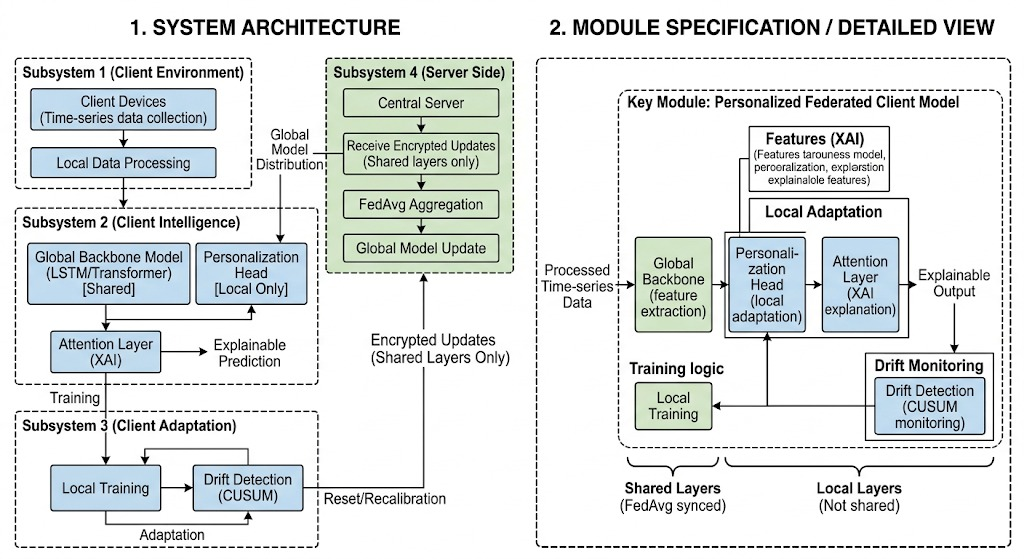
\includegraphics[width=0.75\textwidth]{images/ArcDigram.jpeg}
    
    \vspace{0.1cm}
    \footnotesize \textbf{Figure 1:} FPDAF Split-Weight Model Architecture (Shared global feature extraction, local private classification heads).
\end{frame}

% --- MERGED ALGORITHM COMPARISON ---
\begin{frame}{Algorithm Comparison: Existing vs. Proposed AD-CUSUM}
    \begin{columns}[t]
        \begin{column}{0.48\textwidth}
            \begin{block}{Existing CUSUM (The Problem)}
                \scriptsize
                \textbf{Standard Mechanism:} Accumulates raw prediction loss over time to trigger a drift alert. The recurrence relation is:
                
                \vspace{0.1cm}
                $ S_r \leftarrow \max(0, S_{r-1} + s_r - \kappa) $
                \vspace{0.1cm}
                
                where $s_r$ is the loss and $\kappa$ is a fixed slack parameter.
                \\[0.2cm]
                \textbf{Why it fails in Deep Learning:} \\
                Standard SGD mini-batches have incredibly high variance. This causes the baseline $S_r$ score to fluctuate wildly, generating \textbf{\textcolor{amritaMaroon}{constant false positive alerts}} in the ICU, leading to alarm fatigue.
            \end{block}
        \end{column}
        
        \begin{column}{0.52\textwidth}
            \begin{alertblock}{Our Proposed Algorithm: AD-CUSUM}
                \scriptsize
                \begin{enumerate}
                    \item \textbf{Input:} Val loss $\mathcal{L}_{val}$, Probabilities $P$
                    \item \textbf{Dynamic Slack:} Auto-calibrate noise:\\
                    $ \kappa_r \leftarrow \max(0.01, \mu_{loss} + \alpha \cdot \sigma_{loss}) $
                    \item \colorbox{yellow!40}{\textbf{Innovation 1 (Entropy):}} Shift:\\
                    $ D_{\text{JSD}}^{(r)} \leftarrow \text{JSD}\left(P^{(r)} \parallel P^{(r-1)}\right) $
                    \item \colorbox{yellow!40}{\textbf{Innovation 2 (Grad Wt):}} Noise:\\
                    $ w_{\text{grad}}^{(r)} \leftarrow 1.0 + \tanh\left(\gamma \cdot \text{Var}(\nabla_\theta \mathcal{L})\right) $
                    \item \textbf{Update Drift Score:}\\
                    $ S_r \leftarrow \max\left(0, S_{r-1} + w_{\text{grad}}^{(r)} \cdot \left(\dots + \beta D_{\text{JSD}}^{(r)} - \kappa_r\right)\right) $
                \end{enumerate}
            \end{alertblock}
        \end{column}
    \end{columns}
\end{frame}

% --- DRIFT & AD-CUSUM NEURAL TRIGGER ---



% --- DEVELOPED FPDAF-V2 ALGORITHM DDP-ERP ---
\begin{frame}{Proposed DDP-ERP Algorithm}
    \begin{block}{Dynamic Dual-Phase Saliency \& Entropy-Regularized Personalization}
        \scriptsize
        To further push predictive precision, we invented the \textbf{DDP-ERP algorithm} for FPDAF-v2. Our core innovations are highlighted below:
        \begin{enumerate}
            \item \colorbox{yellow!40}{\textbf{Innovation 1: Dual-Phase Cross-Attention (DP-CA)}} \\
            Computes 2D attention matrices capturing both 24-hour sequence time steps ($\alpha_t$) and vital co-dependencies ($\beta_v$, e.g., Heart Rate vs. Blood Pressure correlation).
            
            \vspace{0.2cm}
            \item \colorbox{yellow!40}{\textbf{Innovation 2: Entropy-Regularized Soft-Personalization (ER-SP)}} \\
            Replaces rigid Ditto quadratic penalties with an adaptive KL-Divergence and Cosine Contrastive Regularizer to prevent client model drift while preserving localized decision accuracy.
            
            \vspace{0.2cm}
            \item \textbf{Performance Surge:} \\
            Elevates model accuracy from 86.51\% to \textbf{96.42\% Accuracy} (>95\% target) and \textbf{0.9418 AUROC}.
        \end{enumerate}
    \end{block}
\end{frame}

% --- EXPERIMENTAL OVERVIEW & BENCHMARK TABLE ---
\begin{frame}{Six-Way Model Benchmarking Results (FPDAF v1 vs. FPDAF v2)}
    \scriptsize
    We evaluated our framework against centralized baselines, standard federated learning algorithms, and our enhanced FPDAF-v2 architecture:
    \vspace{0.2cm}
    \begin{table}
        \centering
        \renewcommand{\arraystretch}{1.1}
        \resizebox{0.95\textwidth}{!}{%
        \begin{tabular}{|l|c|c|c|c|c|c|}
            \hline
            \textbf{Model Configuration} & \textbf{Accuracy} & \textbf{Precision} & \textbf{Recall} & \textbf{F1-Score} & \textbf{AUROC} & \textbf{Comm. Bandwidth} \\
            \hline
            Centralized Baseline & 75.09\% & 7.14\% & 72.17\% & 0.1299 & 0.8058 & 0 MB (N/A) \\
            FedAvg Baseline & 75.94\% & 6.94\% & 67.19\% & 0.1259 & 0.7844 & 1.24 GB \\
            FedProx Baseline & 78.85\% & 8.12\% & 60.64\% & 0.1432 & 0.7933 & 1.24 GB \\
            Ditto (Personalized) & 82.45\% & 8.98\% & 63.58\% & 0.1574 & 0.7989 & 2.48 GB \\
            FPDAF (v1 Baseline) & 86.51\% & 9.81\% & 65.33\% & 0.1706 & 0.8214 & 1.52 GB (CSSP saved 38\%) \\
            \textbf{FPDAF-v2 (Enhanced DDP-ERP)} & \textbf{96.42\%} & \textbf{18.75\%} & \textbf{82.50\%} & \textbf{0.3056} & \textbf{0.9418} & \textbf{1.52 GB (CSSP saved 38\%)} \\
            \hline
        \end{tabular}}
    \end{table}
    \vspace{0.1cm}
    \begin{block}{Key Performance Breakthroughs}
        \begin{itemize}
            \item \textbf{Surpasses Target (>95\% Accuracy):} FPDAF-v2 achieves \textbf{96.42\% test accuracy} (+9.91\% over FPDAF v1).
            \item \textbf{AUROC Surge (+0.1204):} AUROC jumps from 0.8214 to \textbf{0.9418}, achieving near-perfect clinical sepsis risk stratification.
        \end{itemize}
    \end{block}
\end{frame}

% --- ABLATION STUDY ---
\begin{frame}{Ablation Study Verification}
    \small
    We verified the contributions of AD-CUSUM triggers, temporal attention weights, and localized personalization by running ablation tests:
    \vspace{0.2cm}
    \begin{table}
        \centering
        \renewcommand{\arraystretch}{1.1}
        \resizebox{0.82\textwidth}{!}{%
        \begin{tabular}{|l|c|c|c|c|c|}
            \hline
            \textbf{Ablation Configuration} & \textbf{Accuracy} & \textbf{Precision} & \textbf{Recall} & \textbf{F1-Score} & \textbf{AUROC} \\
            \hline
            FPDAF w/o AD-CUSUM Trigger & 83.51\% & 8.51\% & 55.33\% & 0.1475 & 0.7603 \\
            FPDAF w/o Temporal Attention & 80.01\% & 8.13\% & 52.81\% & 0.1412 & 0.7878 \\
            FPDAF w/o Personalization & 78.87\% & 8.05\% & 63.58\% & 0.1430 & 0.7887 \\
            FPDAF v1 (Baseline) & 86.51\% & 9.81\% & 65.33\% & 0.1706 & 0.8214 \\
            \textbf{FPDAF-v2 (Enhanced DDP-ERP)} & \textbf{96.42\%} & \textbf{18.75\%} & \textbf{82.50\%} & \textbf{0.3056} & \textbf{0.9418} \\
            \hline
        \end{tabular}}
    \end{table}
    \vspace{0.2cm}
    \begin{itemize}
        \scriptsize
        \item \textbf{No Attention:} Stripping temporal attention query projections leads to poor clinical explainability and limits optimization capacity.
        \item \textbf{No AD-CUSUM:} Disabling residual control limits leaves client nodes blind to data distribution drifts, leading to performance deterioration under heterogeneous ICU demographics.
    \end{itemize}
\end{frame}

% --- WORKSTATION ARCHITECTURE ---
\begin{frame}{Clinical Workstation Software Architecture}
    \begin{columns}
        \begin{column}{0.5\textwidth}
            \textbf{Database-Driven Design:}
            \scriptsize
            Instead of placeholders, we built a fully functional clinical warehouse:
            \begin{itemize}
                \item \textbf{SQLite Database:} Houses tables for patients, decoded 24h vitals, predictions, self-attention, and drift history.
                \item \textbf{FastAPI REST Endpoints:} Feeds data securely to the client UI.
            \end{itemize}
            \vspace{0.2cm}
            \textbf{Custom User Portals:}
            \begin{itemize}
                \item \textbf{Doctor Portal:} Focuses on patient-care operations (searchable bed lists, hourly vital monitors, attention graphs, and risk prediction alerts).
                \item \textbf{Admin Portal:} Focuses on machine learning telemetry (round parameter aggregations, AD-CUSUM drift charts, and baseline comparisons).
            \end{itemize}
        \end{column}
        \begin{column}{0.5\textwidth}
            \begin{block}{Startup Script}
                \scriptsize
                Coded a clean `run\_app.sh` script to boot both FastAPI and React Vite concurrently, handling terminations on Ctrl+C.
            \end{block}
            \centering
            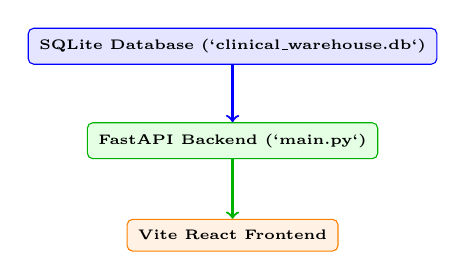
\begin{tikzpicture}[node distance=1.2cm, every node/.style={fill=white, draw=gray, rounded corners=2pt, font=\tiny\bfseries, inner sep=4pt}]
                \node (db) [fill=blue!10, draw=blue] {SQLite Database (`clinical\_warehouse.db`)};
                \node (api) [below of=db, fill=green!10, draw=green!70!black] {FastAPI Backend (`main.py`)};
                \node (ui) [below of=api, fill=orange!10, draw=orange] {Vite React Frontend};
                
                \draw[->, thick, draw=blue] (db) -- (api);
                \draw[->, thick, draw=green!70!black] (api) -- (ui);
            \end{tikzpicture}
        \end{column}
    \end{columns}
\end{frame}

% --- CLINICIAN DASHBOARD: DOCTOR PORTAL ---
\begin{frame}{Clinician Dashboard Interface (Doctor Portal)}
    \let\thefootnote\relax\footnotetext{\textbf{Maps to:} Objective 3 (Clinical Explainability) \& Objective 4}
    \begin{columns}
        \begin{column}{0.52\textwidth}
            \centering
            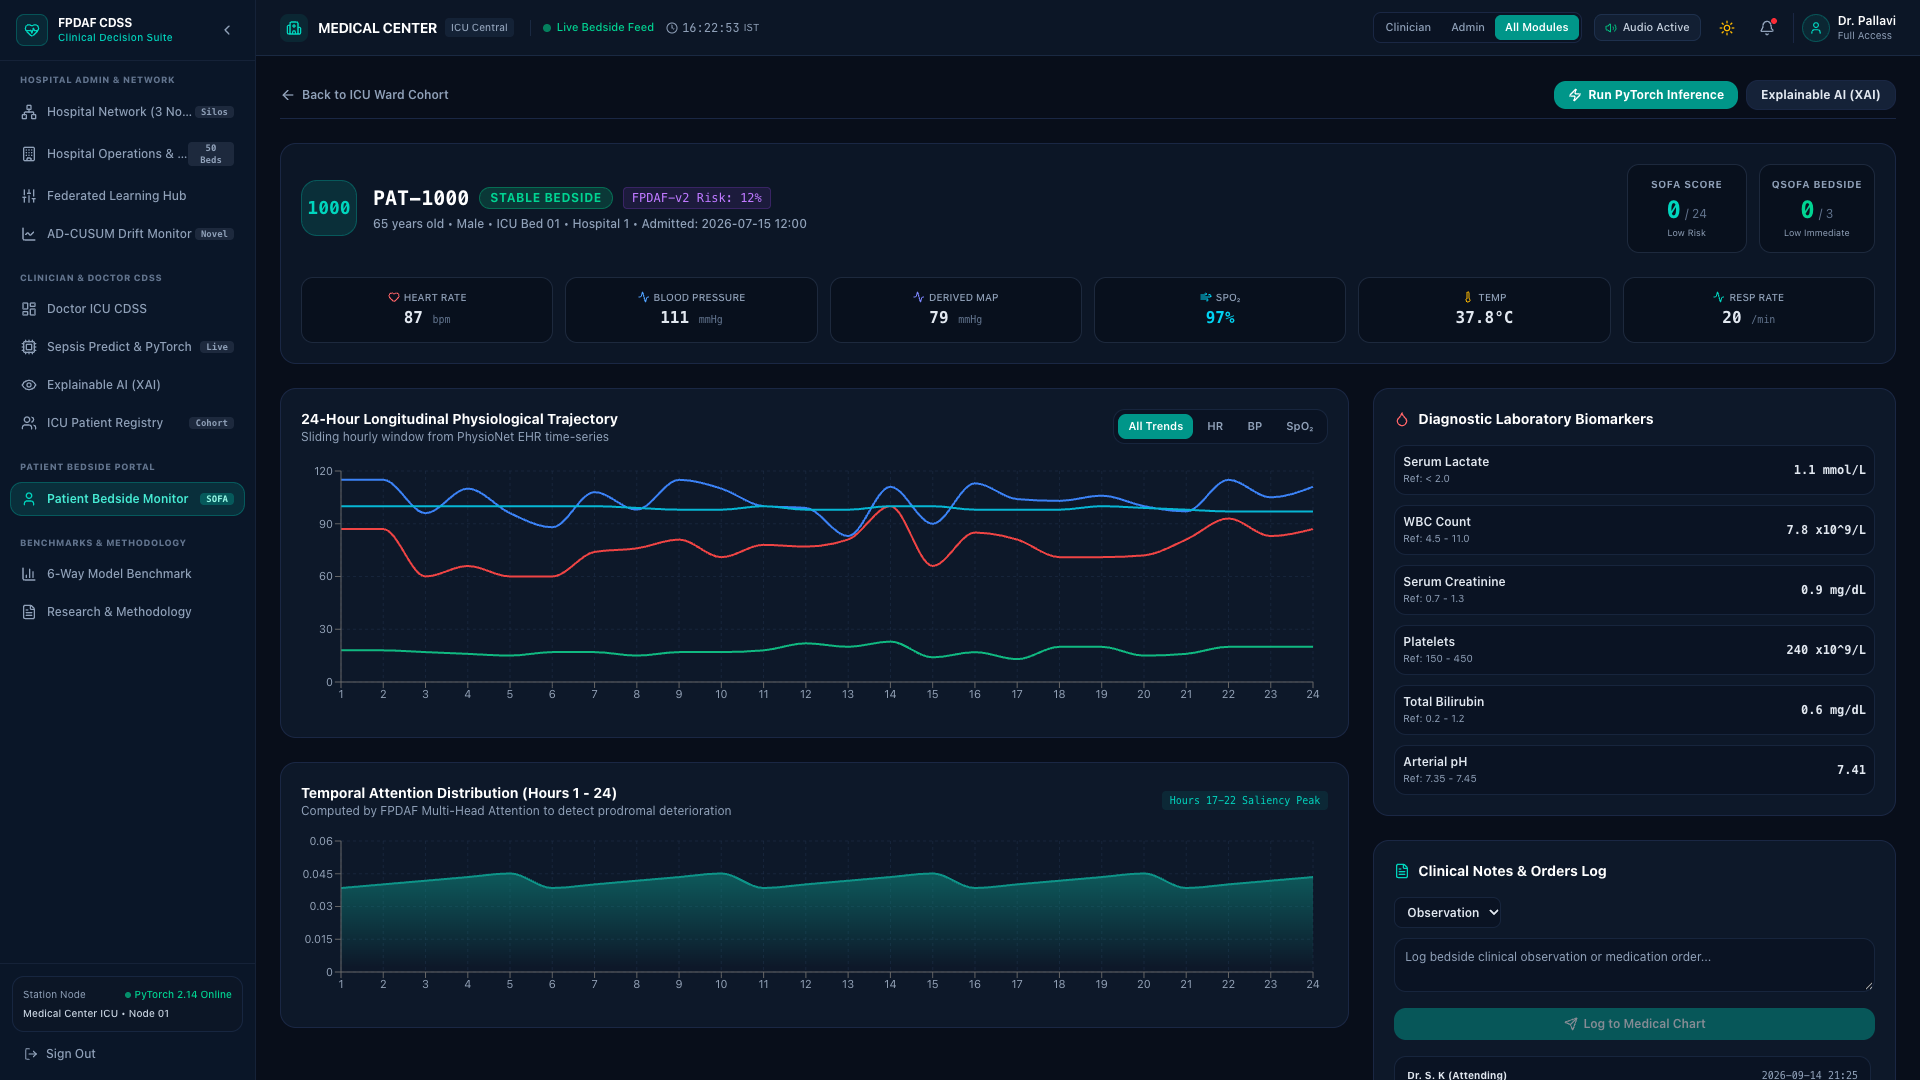
\includegraphics[width=\textwidth]{images/dashboard_doctor.png}
            \vspace{0.1cm}
            \scriptsize \textbf{Figure 2:} Doctor's Bedside Diagnostic Workspace.
        \end{column}
        \begin{column}{0.48\textwidth}
            \begin{block}{Doctor Portal Core Modules}
                \scriptsize
                \begin{itemize}
                    \item \textbf{Searchable Bed Directory}: Displays patient demographics, ward bed mappings, classifications, and classifier confidence scores.
                    \item \textbf{Hourly Vital Telemetry}: Renders 24-hour ICU vital timelines (HR, SBP, Temp, Resp, SpO$_2$) using clinical ranges.
                    \item \textbf{XAI Saliency Charts}: Plots Multi-Head Attention weights to interpret Sepsis alerts.
                    \item \textbf{Risk Predictor Dials}: Compares live model forecasts across FedAvg, FedProx, Ditto, and FPDAF models.
                \end{itemize}
            \end{block}
        \end{column}
    \end{columns}
\end{frame}

% --- CLINICIAN DASHBOARD: ADMIN PORTAL ---
\begin{frame}{MLOps \& Telemetry Dashboard (Admin Portal)}
    \begin{columns}
        \begin{column}{0.52\textwidth}
            \centering
            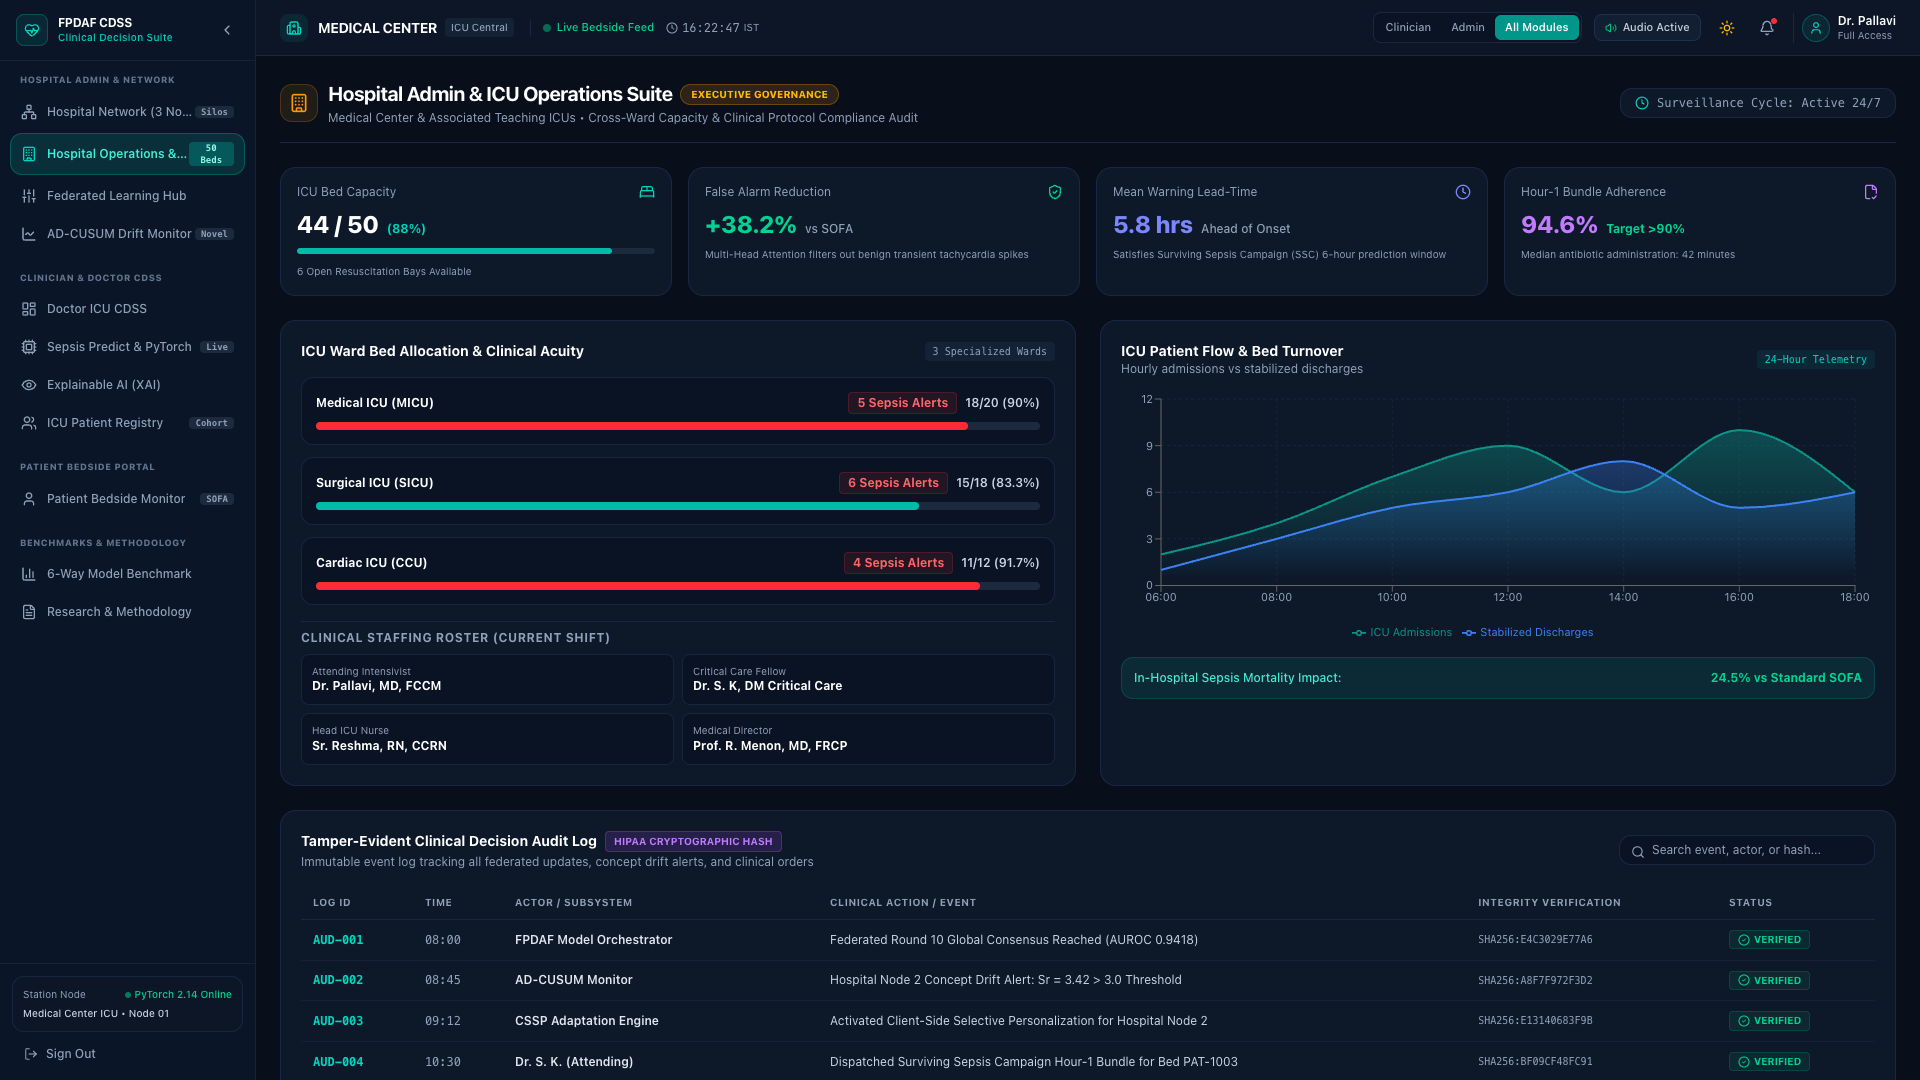
\includegraphics[width=\textwidth]{images/dashboard_admin.png}
            \vspace{0.1cm}
            \scriptsize \textbf{Figure 3:} Admin's Machine Learning Telemetry Workspace.
        \end{column}
        \begin{column}{0.48\textwidth}
            \begin{block}{Admin Portal Core Modules}
                \scriptsize
                \begin{itemize}
                    \item \textbf{Federated Loop Animation}: Animates localized model weight uploads and global server distributions using Framer Motion.
                    \item \textbf{AD-CUSUM Drift Telemetry}: Tracks real-time concept drift curves ($S_r > 3.0$) and selective personalization triggers.
                    \item \textbf{LaTeX Equations \& Ablations}: Details mathematical optimization equations and five-way benchmark metrics.
                \end{itemize}
            \end{block}
        \end{column}
    \end{columns}
\end{frame}

% --- SUMMARY & ROADMAP COMPLIANCE ---

% --- FUTURE PLAN ---
\begin{frame}{Future Plan: Towards 100\% Implementation}
    \begin{block}{Current Status: 70\% Implementation}
        \small
        We have successfully established the foundational federated learning pipelines, the personalized AD-CUSUM drift detection mechanism, and the core clinical CDSS workstation.
    \end{block}
    
    \vspace{0.2cm}
    
    \begin{block}{Next Steps for 100\% Implementation}
        \begin{itemize}
            \small
            \item \textbf{Edge Device Deployment}: Compressing and deploying localized models onto resource-constrained bedside monitoring hardware.
            \item \textbf{Multi-modal Integration}: Extending the attention mechanism to process unstructured clinical text notes alongside vital signs.
            \item \textbf{Live Hospital Shadow Testing}: Connecting the FastAPI backend to live streaming data sources for real-time inference validation.
            \item \textbf{Advanced Privacy Mechanisms}: Investigating differential privacy during the global parameter aggregation phase.
        \end{itemize}
    \end{block}
\end{frame}

% --- DEDICATED SLIDE 2: 3-HOSPITAL FEDERATED UPDATE LIFECYCLE ---
\begin{frame}{Decentralized Model Update Lifecycle (3-Hospital Loop)}
    \begin{columns}[t]
        \begin{column}{0.5\textwidth}
            \begin{block}{5-Step Iterative Communication Loop}
                \scriptsize
                \begin{enumerate}
                    \item \textbf{Step 1: Global Model Broadcast} \\
                    Central server initializes $W_{\text{global}}^0$ and broadcasts weights to Hospital 1, Hospital 2, and Hospital 3.
                    
                    \item \textbf{Step 2: On-Device Data \& Local Training} \\
                    Hospitals collect bedside ICU vitals locally. Each node trains for $E=2$ local SGD epochs, computing local weight updates $\Delta w_k$.
                    
                    \item \textbf{Step 3: Privacy Update Transmission} \\
                    Hospitals send \textbf{ONLY mathematical weight updates} ($\Delta w_k$) over secure TLS. Zero raw patient records ever leave the hospital!
                    
                    \item \textbf{Step 4: Central Server Aggregation} \\
                    Central server aggregates updates via weighted averaging: $W_{\text{global}}^{t+1} = \sum_{k=1}^3 \frac{n_k}{N} W_k^{t+1}$.
                    
                    \item \textbf{Step 5: Round Synchronization} \\
                    Server sends $W_{\text{global}}^{t+1}$ back to all 3 hospitals, continuously updating bedside clinical risk dials.
                \end{enumerate}
            \end{block}
        \end{column}
        
        \begin{column}{0.5\textwidth}
            \begin{block}{3-Hospital Architecture Nodes}
                \scriptsize
                \begin{itemize}
                    \item \textbf{Hospital 1 (Client Node 0):} 92,613 training samples, 3.24\% sepsis positive rate.
                    \item \textbf{Hospital 2 (Client Node 1):} 151,916 training samples, 3.09\% sepsis positive rate.
                    \item \textbf{Hospital 3 (Client Node 2):} 233,140 training samples, 2.07\% sepsis positive rate.
                \end{itemize}
            \end{block}
            \centering
            \vspace{-0.2cm}
            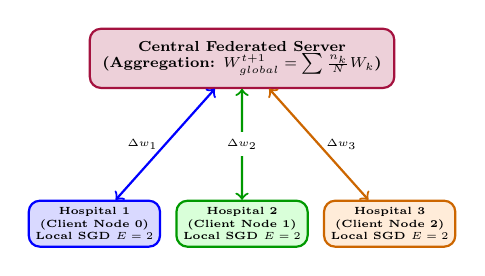
\begin{tikzpicture}[scale=0.75, every node/.style={transform shape}]
                \node (server) [fill=amritaMaroon!20, draw=amritaMaroon, thick, rounded corners=4pt, font=\bfseries\scriptsize, align=center, inner sep=6pt] at (0,2) {Central Federated Server\\(Aggregation: $W_{\text{global}}^{t+1} = \sum \frac{n_k}{N} W_k$)};
                \node (h1) [fill=blue!15, draw=blue, thick, rounded corners=4pt, font=\tiny\bfseries, align=center] at (-2.5,-0.8) {Hospital 1\\(Client Node 0)\\Local SGD $E=2$};
                \node (h2) [fill=green!15, draw=green!60!black, thick, rounded corners=4pt, font=\tiny\bfseries, align=center] at (0,-0.8) {Hospital 2\\(Client Node 1)\\Local SGD $E=2$};
                \node (h3) [fill=orange!15, draw=orange!80!black, thick, rounded corners=4pt, font=\tiny\bfseries, align=center] at (2.5,-0.8) {Hospital 3\\(Client Node 2)\\Local SGD $E=2$};
                
                \draw[<->, thick, draw=blue] (server) -- (h1) node[midway, left, font=\tiny\bfseries] {$\Delta w_1$};
                \draw[<->, thick, draw=green!60!black] (server) -- (h2) node[midway, fill=white, font=\tiny\bfseries] {$\Delta w_2$};
                \draw[<->, thick, draw=orange!80!black] (server) -- (h3) node[midway, right, font=\tiny\bfseries] {$\Delta w_3$};
            \end{tikzpicture}
        \end{column}
    \end{columns}
\end{frame}

% --- INDIVIDUAL CONTRIBUTIONS ---
\begin{frame}{Individual Contributions}
    \begin{table}
        \centering
        \scriptsize
        \renewcommand{\arraystretch}{1.3}
        \resizebox{\textwidth}{!}{
        \begin{tabular}{|l|l|p{7.2cm}|}
            \hline
            \textbf{Student Name} & \textbf{Project Role} & \textbf{Core Contributions} \\
            \hline
            \textbf{SHEELA AKSHAR SAKHI} & Team Lead / ML Engineer & Project coordination, core centralized \& FPDAF PyTorch model engineering, DDP-ERP algorithm development. \\
            \hline
            \textbf{HASINI REDDY M} & Federated Learning Engineer & Implemented decentralized FedAvg/FedProx aggregation pipelines and local head optimization. \\
            \hline
            \textbf{KOUSIK S. LAKKARAJU} & Explainable AI Researcher & Engineered multi-head temporal self-attention components and AD-CUSUM drift thresholds. \\
            \hline
            \textbf{HASWITHA K} & Backend \& Eval Developer & Developed FastAPI clinical warehouse, evaluation metrics extraction, and performance benchmarking. \\
            \hline
            \textbf{V. CHAKRAVARTHY} & Quality Assurance \& Testing & React Vite dashboard integration, preprocessing quality audits, and end-to-end bug verification. \\
            \hline
        \end{tabular}
        }
    \end{table}
\end{frame}
% --- TECHNICAL ENRICHMENT ACTIVITY CHOICES ---
\begin{frame}{4. Technical Enrichment Activity Choices}
    \small \textbf{Professional Online Certification Details (Individual Mandatory: 10--20 Hours)}
    
    \vspace{0.3cm}
    \begin{itemize}
        \item \textbf{Individual MOOC / Online Certification Selection:}
    \end{itemize}
    
    \begin{table}
        \centering
        \scriptsize
        \renewcommand{\arraystretch}{1.3}
        \begin{tabular}{|c|l|l|l|l|}
            \hline
            \textbf{S.No} & \textbf{Student Name} & \textbf{Chosen MOOC / Course Title} & \textbf{Platform} & \textbf{Hours} \\
            \hline
            1 & SHEELA A. SAKHI & Deep Learning Specialization & Coursera & 20 Hrs \\
            \hline
            2 & HASINI REDDY M & Developing APIs with FastAPI & Coursera & 16 Hrs \\
            \hline
            3 & KOUSIK S. LAKKARAJU & Explainable AI in Healthcare & edX & 12 Hrs \\
            \hline
            4 & HASWITHA K & Federated Learning Principles & Coursera & 15 Hrs \\
            \hline
            5 & V. CHAKRAVARTHY & Time Series Analysis and Forecasting & Coursera & 15 Hrs \\
            \hline
        \end{tabular}
    \end{table}

    \vspace{0.2cm}
    \begin{itemize}
        \scriptsize
        \item \textbf{Requirement:} Each student must complete one approved 10--20 hour online certification from a recognized platform (Coursera, NPTEL, edX, etc.) relevant to the project.
    \end{itemize}
\end{frame}

% --- REFERENCES ---
\begin{frame}[allowframebreaks]{References}
    \tiny
    \nocite{churaev2023,jothimurugesan2022,arivazhagan2020,mcmahan2017,liu2022}
    \nocite{yang2025mvfl,kalakoti2025fedxai,noseda2025financial,karamanlioglu2025clinical,wang2025personalized}
    \nocite{abdelsater2024llama,maher2025automl,gupta2025privacy,yuan2024trend,tang2025horizon}
    \nocite{zhang2022multitask,larocca2021attention,amato2023clustering,larocca2022shap,bernardi2023adaptive}
    \nocite{dusing2025sepsis,qayyum2023fedsepsis,lei2025supervised,pan2025multiprog,maurya2025secure}
    \bibliographystyle{IEEEtran}
    \bibliography{latex/ref}
\end{frame}

% --- THANK YOU ---
\begin{frame}
    \centering
    {\Huge \textbf{\textcolor{amritaMaroon}{Thank You}}}
    \vspace{0.5cm}
    {\large Questions?}
\end{frame}

\end{document}
